While the world grapples with the effects of climate change, the demand for clean and firm energy continues to increase. Utilities and decision-makers face rising energy demands of machine learning and data center companies, which require a constant and reliable energy source. The escalation of data center demand and electrification in the economy has led the \gls{eia} to forego publishing its annual energy outlook report in 2023 as it evaluates its models under emergent market pressures \cite{eia_annual_outlook_canceled_2023}. New nuclear reactors---designed to be more efficient, flexible, and resilient than the reactors that have come before them---can provide clean, firm energy to meet these demands.

Since 1959, the \gls{usa} has commercially operated large \gls{lwr} designs at
nuclear power plants. These reactors use light water as a coolant and moderator
and can be categorized as either \glspl{pwr} or \glspl{bwr}. As shown in Figure
\ref{fig:online_lwr_cap_2024}, the \gls{lwr} fleet in the \gls{usa} expanded power capacity over roughly 20 years before achieving just over 99 GWe in
1990 and remained roughly constant in the years since then. With the recent
connection of Vogtle Units 3 and 4 to the grid, the \gls{usa} has seen the
first new \gls{lwr} units come online in 8 years--following the completion of
Watts Bar-2 in 2016.

\begin{figure}[H]
    \centering
    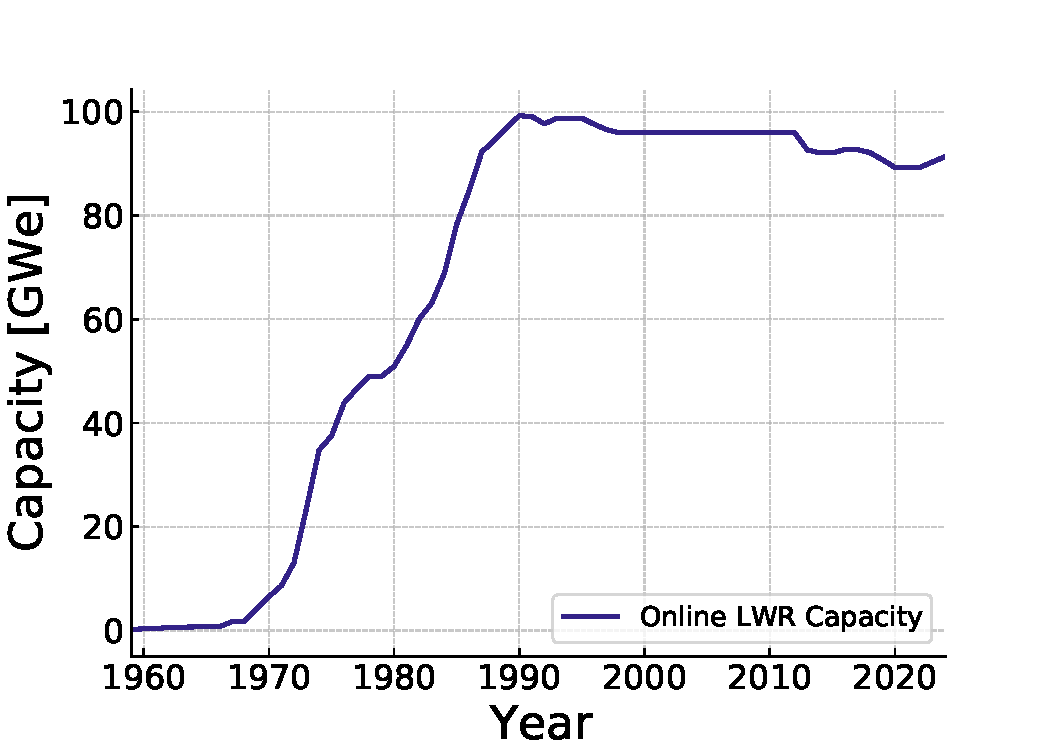
\includegraphics[scale=0.7]{images/intro/online_lwr_cap_2024.pdf}
    \caption{US LWR capacity through 2024. Reproduced from \cite{IAEA_PRIS}.}
    \label{fig:online_lwr_cap_2024}
\end{figure}

According to the \gls{eia}, nuclear power plants produced 18\% of utility-scale
electricity generation in 2023 \cite{eia_elec_gen_2024}, meaning nuclear energy
was 46.5\% of total clean energy generation and the largest clean energy source
in the country. The last license in the fleet will now expire in 2063 following
the completion of Vogtle Unit 4; however, to meet growing energy demands,
the \gls{usa} will need to replace and expand the current fleet as it retires
over that time; deploying new reactors at a rate that has not been seen since
the 1970s. The \gls{doe} has published a liftoff report on how nuclear energy
can expand to meet future demands and has outlined myriad scenarios that could
lead to a 100\% net zero carbon by 2050 \cite{julie_liftoff_pathways_2024}. One
of the striking takeaways from the liftoff report is the necessity of tripling
nuclear energy demand by 2050 due to new capacity demand, the retirement of
fossil fuels, electrification of the economy, and other behind-the-meter
applications of nuclear technologies. The future \gls{doe} outlines is not
without its challenges; the \gls{eia} 2023 Domestic Uranium Production Report
highlights the decrease in uranium concentrate production in the \gls{usa} and
the number of fuel cycle facilities that are dormant or have been
decommissioned \cite{eia_uranium_statistics_2023}.

Despite these deployment challenges, the \gls{doe} liftoff report asserts that
high-value propositions in low land use, firm energy generation, direct heat
applications, local economic benefits, and the low transmission build-out
associated with nuclear energy make it a compelling choice. Some of these
benefits can be reflected in the 73\% increase in uranium production workers
from 2022 to 2023, the 4x increase in exploration of uranium resources, and a
\$20 million increase in resource investment \cite{eia_uranium_statistics_2023}
---the private sector is starting to move on the value proposition of nuclear energy.

The current fleet of \glspl{lwr} has been the backbone of the commercial nuclear
industry, but the industry is on the precipice of a different generation of
reactor technologies. The fleet of \glspl{lwr} uses a ceramic uranium-oxide fuel
that is enriched to 3-5\% $^{235}$U, but there is a panoply of advanced reactor
designs at various stages of deployment using decades of
experience with creating nuclear energy. These reactors vary in size from large
gigawatt-scale reactors to smaller reactors designed to fit on the back of a
truck. The design space is vast, but one innovation that has been a focus of
the nuclear industry is the \gls{triso} fuel particle. This fuel particle is a small sphere of uranium fuel coated in carbon and silicon carbide layers. \gls{triso} is designed to be more robust than traditional fuel and to be used in various reactor designs that require \gls{haleu} (5-20\%).

The \gls{nfc} describes the steps nuclear fuel goes through
in its life cycle. Figure \ref{fig:once-through} outlines a simple \textit{once-through} fuel cycle (so-called because the fuel goes through the cycle once in its lifetime). The fuel cycle begins with mining uranium ore, typically from uraninite or pitchblende deposits. Then, the ore must be milled and refined into yellowcake, which can then be converted into uranium hexafluoride. To power the reactors in the \gls{usa}, the uranium hexafluoride is then enriched to the desired percentage of $^{235}$U and converted into uranium dioxide. Reactor operators receive the fuel in rods after it has been fabricated into fuel pellets from uranium dioxide. Upon receiving the fuel, workers load the rods into the reactor to generate heat. The heat generates steam, which drives a turbine and generates electricity. After years of operation, workers remove the used fuel from the reactor and store it in a spent fuel pool. After cooling, transporters move the used fuel to dry cask storage, where it will remain until policymakers act to enable a long-term solution.

\begin{figure}[H]
    \centering
    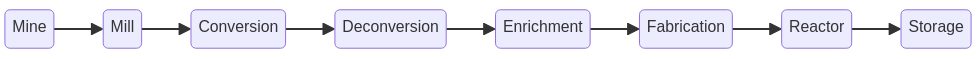
\includegraphics[scale=0.40]{images/once_through_fc.png}
    \caption{US once-through fuel cycle.}
    \label{fig:once-through}
\end{figure}

Although linear in \ref{fig:once-through}, in reality these steps are interwoven with multilateral relationships and long-term purchasing agreements that complicate the establishment of new supply chains. Consequently, the availability of services at each step in the fuel cycle is difficult to model; this is where the \cyclus \cite{huff_cyclus_intro_2016} tool is valuable. \cyclus is a nuclear fuel cycle simulator that allows users to model the material movement between facilities in discrete-event simulations. These facilities are run by agents that make decisions and interact with other agents. Because \cyclus is designed to be technology agnostic, it can model a variety of fuel cycles and reactor types--although it is not primarily a physics engine, so coupling it with physics software can be necessary for some problems.

Partners in industry, academia, and government are building the body of
literature surrounding \gls{triso} fuel cycles. This thesis is a timely
evaluation of various energy-demand scenarios and an optimization of the
deployment of advanced reactors building off of the method established by
Bachmann et al. \cite{bachmann_enrichment_2021} for \gls{haleu} fuel,
incorporating a phased enrichment demand that advanced reactor companies could
explore as the \gls{haleu} supply chain develops. This thesis seeks to
understand the potential for advanced reactor deployment in the \gls{usa} and
the implications of the fuel cycle on the deployment of these reactors, as some
designs adopt a staggered enrichment demand for various \gls{triso} fuels. This thesis will focus on \gls{swu}, energy output, mass of fuel, and reactor deployment to understand the performance of each deployment scenario. In service of this goal, this thesis will also examine the computational efficiency of the \gls{dre} in \cyclus to contribute to a robust tool for future analysis.


The structure of this thesis is as follows:

\begin{itemize}
    \item Chapter 2 outlines energy system modeling, the reactors investigated in this thesis, the types of fuel, and the \cyclus tool as it pertains to this thesis.
    \item Chapter 3 discusses the deployment schemes analyzed in this thesis, the metrics used to evaluate the scenarios, and presents the results of each.
    \item Chapter 4 outlines two reactor archetypes developed in this thesis, and compares them to the \cycamore reactor.
    \item Chapter 5 concludes the work in Chapters 3 and 4, discusses the assumptions and limitations, and presents directions for future work.
    \item Appendix A shows the details for each reactor in the "existing fleet" from this thesis.
    \item Appendix B discusses the reactor deployment schemes that were not used in this thesis.
    \item Appendix C discusses the availability and reproducibility of this thesis.
\end{itemize}